% 一维波动方程的数值解
% 波动方程|边界条件|有限差分

\pentry{一维波动方程\upref{WEq1D}, Matlab 的判断与循环\upref{MIfFor}}

\footnote{本文参考了 \href{http://hplgit.github.io/num-methods-for-PDEs/doc/pub/wave/sphinx/._main_wave001.html\#discretizing-the-domain}{BCB}}已知一维的波动方程为(\autoref{WEq1D_eq3}~\upref{WEq1D})

\begin{equation}
\pdv[2]{y}{x} - \frac{1}{c^2}\pdv[2]{y}{t} = 0
\end{equation}

其中 $y(x, t)$ 是坐标和时间的函数. 这里介绍一个简单的\textbf{有限差分(finite difference)}法, 即把空间 $x$ 和时间 $t$ 划分成等距离的网格 $x_1, \dots, x_{Nx}$ 和 $t_1, \dots, t_{Nt}$, 步长分别为 $\Delta x$ 和 $\Delta t$. 我们将每个格点处的函数值记为 $y_{i,n} = y(x_i, t_n)$

有了网格以后, 我们可以用有限差分表示二阶导数(\autoref{DerDif_eq5}~\upref{DerDif})得
\begin{equation}
\frac{y_{i-1,n} - 2y_{i,n} + y_{i+1,n}}{\Delta x^2} - \frac{1}{c^2} \frac{y_{i, n-1} - 2y_{i, n} + y_{i, n+1}}{\Delta t^2} = 0
\end{equation}
整理得
\begin{equation}
y_{i, n+1} = 2y_{i, n} - y_{i, n-1} + C^2(y_{i-1,n} - 2y_{i,n} + y_{i+1,n})
\end{equation}
其中
\begin{equation}
C = c \frac{\Delta t}{\Delta x}
\end{equation}
是一个无量纲得常数. 也就是说, 当我们已知 $t_n$ 和 $t_{n-1}$ 时刻的波函数, 就可以得到 $t_{n+1}$ 时刻的波函数.

\subsection{边界条件}
如果令网格边界处 $y = 0$ (Dirichlet 边界条件) 则会发生全反射且有半波损失. 若边界处使用 $\pdv*{y}{x} = 0$(Neumann 边界条件) 同样会发生全反射但没有半波损失.

另外有一种很有用的边界条件叫 open boundary condition 或者 radiation boundary condition\footnote{\href{http://hplgit.github.io/num-methods-for-PDEs/doc/pub/wave/sphinx/._main_wave003.html\#problem-11-implement-open-boundary-conditions}{查看原文}}, 可以使波动完全不发生反射
\begin{equation}
\pdv{y}{t} + c\pdv{y}{x} = 0
\end{equation}
要验证该条件, 将任何速度为 $c$ 的平面波代入发现都可以满足.

\subsection{Matlab 程序}
程序如下, 运行结果(动画)见 \href{http://wuli.wiki/apps/wavBC.html}{wuli.wiki/apps/wavBC.html}. 截图见\autoref{W1dNum_fig1}.

\begin{lstlisting}[language=matlab, caption=wave1D.m]
% 一维波动方程数值解
% 参考 http://wuli.wiki/online/W1dNum.html

function wave1D
close all;

% ==== 参数 ====
c = 1; % 波速
xmin = -4; xmax = 6; Nx = 1200; % 空间格点
tmin = 0; tmax = 12; Nt = 2401; % 时间格点
k = 6; Ncyc = 5; % 初始波包的波数和周期数
bc = 'd'; % 边界条件: [d] Dirichlet, [n] Neumann, [o] Open
% ================

x = linspace(xmin, xmax, Nx)';
t = linspace(tmin, tmax, Nt);
dx = (xmax - xmin)/(Nx - 1);
dt = (tmax - tmin)/(Nt - 1);
C = c*dt/dx; C2 = C*C;
y = zeros(Nx, Nt);
y(:,1) = y0(x, k, Ncyc);
y(:,2) = y0(x - c*dt, k, Ncyc);

% 二阶差分(边界元设为 0)
D2 = @(v) [0;
    v(1:end-2) - 2*v(2:end-1) + v(3:end);
    0];

figure;
for n = 2:Nt - 1
    y(:,n+1) = 2*y(:,n) - y(:,n-1) + C2*D2(y(:,n));
    y = bc_set(y, n+1, bc, c, dx, dt);
    if (mod(n, 8) == 0)
        clf; plot(x, y(:,n+1)); axis([xmin,xmax,-2,2]);
        hold on; scatter([xmin,xmax], [y(1,n+1), y(end,n+1)]);
        if bc == 'd'
            title(['Dirichlet B.C.  t = ', num2str(t(n+1), '%.2f')]);
        elseif bc == 'n'
            title(['Neumann B.C.  t = ', num2str(t(n+1), '%.2f')]);
        else
            title(['Open B.C.  t = ', num2str(t(n+1), '%.2f')]);
        end
        xlabel x; ylabel y;
        drawnow;
        % saveas(gcf, [bc 'wv' num2str(n) '.png']); % 保存图片文件
    end
end
end

% 初始波包
% sin^2 波形
function y = y0(x, k, Ncyc)
T = 2*pi/k;
L = T*Ncyc/2;
y = zeros(size(x));
k0 = k / Ncyc / 2;
for i = 1:numel(x)
    xx = x(i);
    if abs(xx) <= L
        y(i) = cos(k0*xx)^2 * sin(k*xx);
    end
end
end

% 处理边界值
function y = bc_set(y, n, bc, c, dx, dt)
if bc == 'd' % Dirichlet
    y(1, n) = 0;
    y(end, n) = 0;
elseif bc == 'n' % Neumann
    y(1, n) = y(2, n);
    y(end, n) = y(end-1, n);
elseif bc == 'o' % Open
    y(end, n) = y(end-1, n) - 1/c * (y(end-1, n) - y(end-1, n-1))*dx/dt;
end
end
\end{lstlisting}

\begin{figure}[ht]
\centering
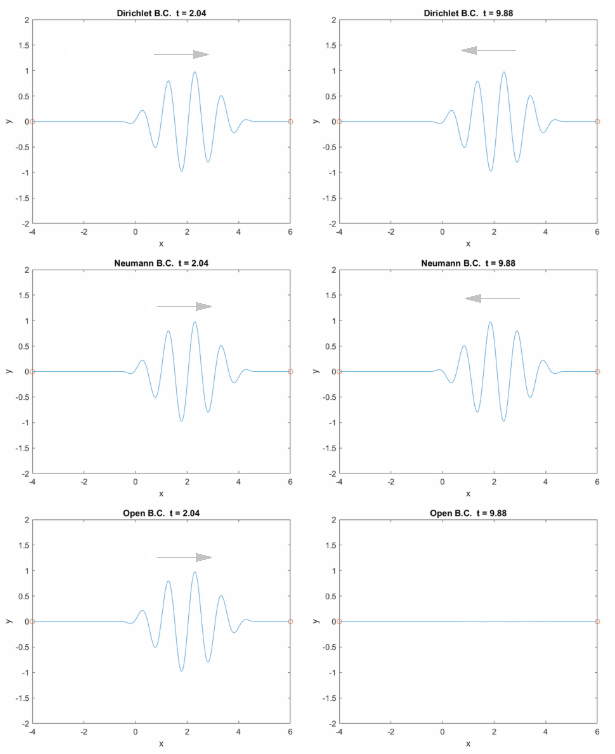
\includegraphics[width=14.25cm]{./figures/W1dNum_1.png}
\caption{运行结果截图, Dirichlet 边界反射后发生相位反转(半波损失), Neumann 边界条件反射后无半波损失, Open 边界条件无反射} \label{W1dNum_fig1}
\end{figure}
